\chapter{Background and Motivation} \label{sec:background-and-motivation}

This chapter introduces the background needed to understand the rest of the thesis. We first review how tensor computations are expressed, how sparse tensors are stored, and how sparse tensor programs are implemented through traversal, merging, and computation. We then distinguish sparse-sparse operations, which require coordinate merging, from sparse-dense operations, which often reduce to scan-and-lookup followed by dense computation. Finally, we review representative scientific computing and machine learning workloads that expose these patterns.

%%%%%%%%%%%%%%%%%%%%%%%%%%%%%%%%%%%%%%%%%%%%%%%%%%%%%%%%%%%%%%%%%%%%%%%%%%%%%%%%%%%%%%%%%%%%%%%%%%%%%%%%%%%%%%%%%%%%%%%%%%%%%%%%%%%
\section{Sparse Tensor Algebra Fundamentals} \label{sec:sparse-tensor-algebra-fundamentals} %%%%%%%%%%%%%%%%%%%%%%%%%%%%%%%%%%%%%%%
%%%%%%%%%%%%%%%%%%%%%%%%%%%%%%%%%%%%%%%%%%%%%%%%%%%%%%%%%%%%%%%%%%%%%%%%%%%%%%%%%%%%%%%%%%%%%%%%%%%%%%%%%%%%%%%%%%%%%%%%%%%%%%%%%%%

Tensor algebra expresses computations over tensors. An \emph{order}-\textit{n} tensor is an \textit{n}-dimensional collection of data; for example, $A_{ijk}$ denotes the scalar element at position $(i,j,k)$ of an order-3 tensor $A$. A widely used way of describing tensor computation, particularly in machine learning frameworks such as PyTorch~\cite{pytorch2019neurips}, is through Einsum expressions~\cite{taco2017oopsla}.

%%%%%%%%%%%%%%%%%%%%%%%%%%%%%%%%%%%%%%%%%%%%%%%%%%%%%%%%%%%%%%%%%%%%%%%%%%%%%%%%%%%%%%%%%%%%%%%%%%%%%%%%%%%%%%%%%%%%%%%%%%%%%%%%%%%
\subsection{Einsum Expressions} \label{sec:einsum-expressions} %%%%%%%%%%%%%%%%%%%%%%%%%%%%%%%%%%%%%%%%%%%%%%%%%%%%%%%%%%%%%%%%%%%%
%%%%%%%%%%%%%%%%%%%%%%%%%%%%%%%%%%%%%%%%%%%%%%%%%%%%%%%%%%%%%%%%%%%%%%%%%%%%%%%%%%%%%%%%%%%%%%%%%%%%%%%%%%%%%%%%%%%%%%%%%%%%%%%%%%%

Einsum expressions specify tensor computations by describing how input and output dimensions relate: (i) input dimensions with repeated indices are combined \emph{element-wise}, (ii) input dimensions whose index is absent from the output are \emph{contracted}, and (iii) all other dimensions are copied to the output. For instance, matrix--vector multiplication is expressed as $Z_i = A_{ij} B_j$. Because the index $j$ does not appear in the output, it is contracted (i.e., multiplied element-wise and summed). Similarly, matrix multiplication is $Z_{ij} = A_{ik} B_{kj}$, contracting along $k$. By contrast, matrix addition is written as $Z_{ij} = A_{ij} + B_{ij}$, expressing element-wise addition across all coordinates.

These expressions are implemented in software as deep loop nests, where each loop iterates over and combines tensor \emph{fibers}---one-dimensional views of a tensor (e.g., matrix rows or columns)~\cite{tacoscheduling2020oopsla}. The loop order is determined by an index \textit{schedule}~\cite{taco2017oopsla}. For example, an inner-product implementation of matrix multiplication uses the schedule $ijk$, an outer-product implementation uses $kij$, and a dataflow implementation uses $ikj$~\cite{gao2023spgemm_survey}. However, the iteration bounds of these loops depend on the compression format in which input tensors are stored~\cite{chou2018abstraction}, as discussed next.

%%%%%%%%%%%%%%%%%%%%%%%%%%%%%%%%%%%%%%%%%%%%%%%%%%%%%%%%%%%%%%%%%%%%%%%%%%%%%%%%%%%%%%%%%%%%%%%%%%%%%%%%%%%%%%%%%%%%%%%%%%%%%%%%%%%
\subsection{Tensor Compression Formats} \label{sec:tensor-compression-formats} %%%%%%%%%%%%%%%%%%%%%%%%%%%%%%%%%%%%%%%%%%%%%%%%%%%%
%%%%%%%%%%%%%%%%%%%%%%%%%%%%%%%%%%%%%%%%%%%%%%%%%%%%%%%%%%%%%%%%%%%%%%%%%%%%%%%%%%%%%%%%%%%%%%%%%%%%%%%%%%%%%%%%%%%%%%%%%%%%%%%%%%%

\begin{figure}
\centering
  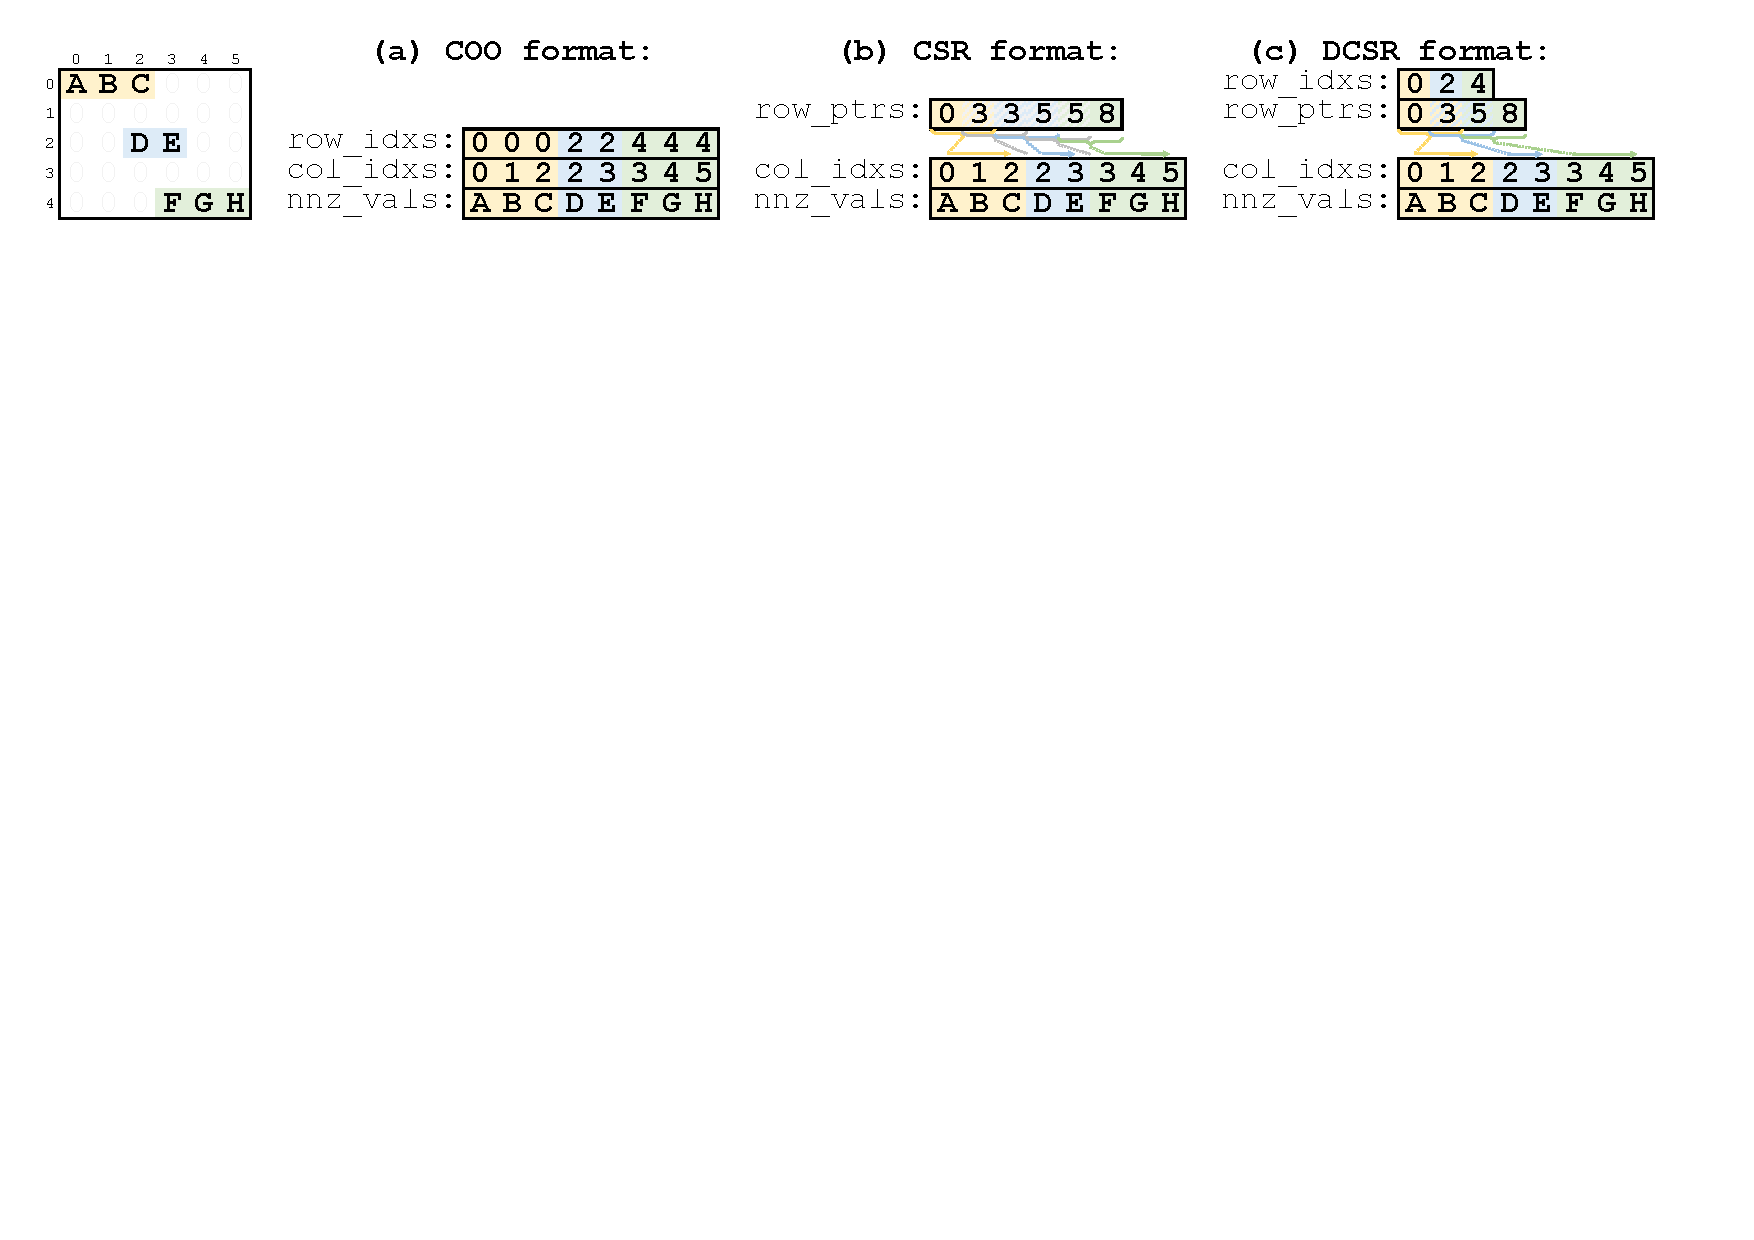
\includegraphics[width=\textwidth]{img_matrix_formats.pdf}
  \caption[Sparse tensor compression formats.]{A sparse matrix and its representation in three common tensor compression formats. The Coordinate (COO) format explicitly stores nonzero elements and their coordinates. The Compressed Sparse Row (CSR) format compresses the row indices by storing only the pointers indicating where each row begins in the vectors that store column indices and nonzero values. The Doubly-Compressed Sparse Row (DCSR) format also compresses the row pointers by storing the index of each nonempty row and its pointer.}
  \label{fig:sparse_formats}
\end{figure}

Dense tensors store their fibers contiguously according to a specified data layout (e.g., row- or column-major). Sparse tensors instead rely on compressed formats that store only nonzero values (\emph{nnzs}) and their coordinates. \Cref{fig:sparse_formats} summarizes several widely used sparse matrix formats~\cite{chou2018abstraction}. Specifically:
\begin{enumerate}[label=(\alph*)]
    \item The Coordinate (COO) format (\Cref{fig:sparse_formats}a) explicitly stores nonzero positions as $n$-dimensional coordinates---\texttt{row\_idxs} and \texttt{col\_idxs} for matrices---typically sorted by a multidimensional ordering (e.g., row-major).
    \item For matrices with $\#nnzs > \#rows + 1$, the Compressed Sparse Row (CSR) format~\cite{barret94csr} (\Cref{fig:sparse_formats}b) improves upon COO by storing row boundaries in a \texttt{row\_ptrs} array, eliminating repeated row indices. Therefore, in the CSR format, the \texttt{col\_idxs} vector stores the column indices of its nonzero elements. The \texttt{row\_ptrs} vector stores the position at which each row begins.
    \item When $\#rows \gg \#nonempty\_rows$, the Doubly-Compressed Sparse Row (DCSR) format~\cite{buluc2008dcsr} (\Cref{fig:sparse_formats}c) further compresses the \texttt{row\_ptrs} by omitting empty rows.
\end{enumerate}
Higher-dimensional tensors are typically stored either in COO or in Compressed Sparse Fiber (CSF)~\cite{smith2015csf}, a generalization of DCSR that compresses fibers at each tensor dimension.

Chou et al.~\cite{chou2018abstraction} formalize a hierarchical abstraction for expressing these formats using six \textit{level formats}. For example,
\begin{itemize}
    \item CSR can be represented as a \textit{dense} level followed by a \textit{compressed} level,
    \item DCSR requires two compressed levels,
    \item COO is expressed as a set of \textit{singleton} levels, one per dimension,
    \item CSF is expressed as a hierarchy of compressed levels.
\end{itemize}
This abstraction enables the construction of arbitrarily complex formats, allowing developers to tune performance and storage efficiency for specific algorithms~\cite{taco2017oopsla}.

%%%%%%%%%%%%%%%%%%%%%%%%%%%%%%%%%%%%%%%%%%%%%%%%%%%%%%%%%%%%%%%%%%%%%%%%%%%%%%%%%%%%%%%%%%%%%%%%%%%%%%%%%%%%%%%%%%%%%%%%%%%%%%%%%%%
\subsection{Tensor Traversal} \label{sec:tensor-traversal} %%%%%%%%%%%%%%%%%%%%%%%%%%%%%%%%%%%%%%%%%%%%%%%%%%%%%%%%%%%%%%%%%%%%%%%%%%
%%%%%%%%%%%%%%%%%%%%%%%%%%%%%%%%%%%%%%%%%%%%%%%%%%%%%%%%%%%%%%%%%%%%%%%%%%%%%%%%%%%%%%%%%%%%%%%%%%%%%%%%%%%%%%%%%%%%%%%%%%%%%%%%%%%

Each level format defines a specific \emph{traversal} (i.e., iteration and loading) method, such as:
\begin{enumerate}
\item Dense traversal:
\begin{small}
\begin{verbatim}
for(idx = 0; idx < fbrSize; idx++)
  val = vals[idx];
\end{verbatim}
\end{small}

\item Compressed traversal:
\begin{small}
\begin{verbatim}
for(p = ptr[i]; p < ptr[i+1]; p++) {
  idx = idxs[p];
  val = vals[p];
}
\end{verbatim}
\end{small}

\item Coordinate singleton traversal:
\begin{small}
\begin{verbatim}
for(p = 0; p < numNnzs; p++) {
  idx0 = idxs0[p];
  idx1 = idxs1[p];
  val = vals[p];
}
\end{verbatim}
\end{small}
\end{enumerate}

Tensor traversal is implemented by nesting these level-specific functions into deep loop hierarchies. To perform computation, multiple tensors are often co-iterated and combined, typically at the fiber level. For example, summing two tensors requires co-iterating their fibers and adding elements with matching coordinates.

%%%%%%%%%%%%%%%%%%%%%%%%%%%%%%%%%%%%%%%%%%%%%%%%%%%%%%%%%%%%%%%%%%%%%%%%%%%%%%%%%%%%%%%%%%%%%%%%%%%%%%%%%%%%%%%%%%%%%%%%%%%%%%%%%%%
\subsection{Tensor Merging} \label{sec:tensor-merging} %%%%%%%%%%%%%%%%%%%%%%%%%%%%%%%%%%%%%%%%%%%%%%%%%%%%%%%%%%%%%%%%%%%%%%%%%%%%%%
%%%%%%%%%%%%%%%%%%%%%%%%%%%%%%%%%%%%%%%%%%%%%%%%%%%%%%%%%%%%%%%%%%%%%%%%%%%%%%%%%%%%%%%%%%%%%%%%%%%%%%%%%%%%%%%%%%%%%%%%%%%%%%%%%%%

\begin{figure}[]
\centering
  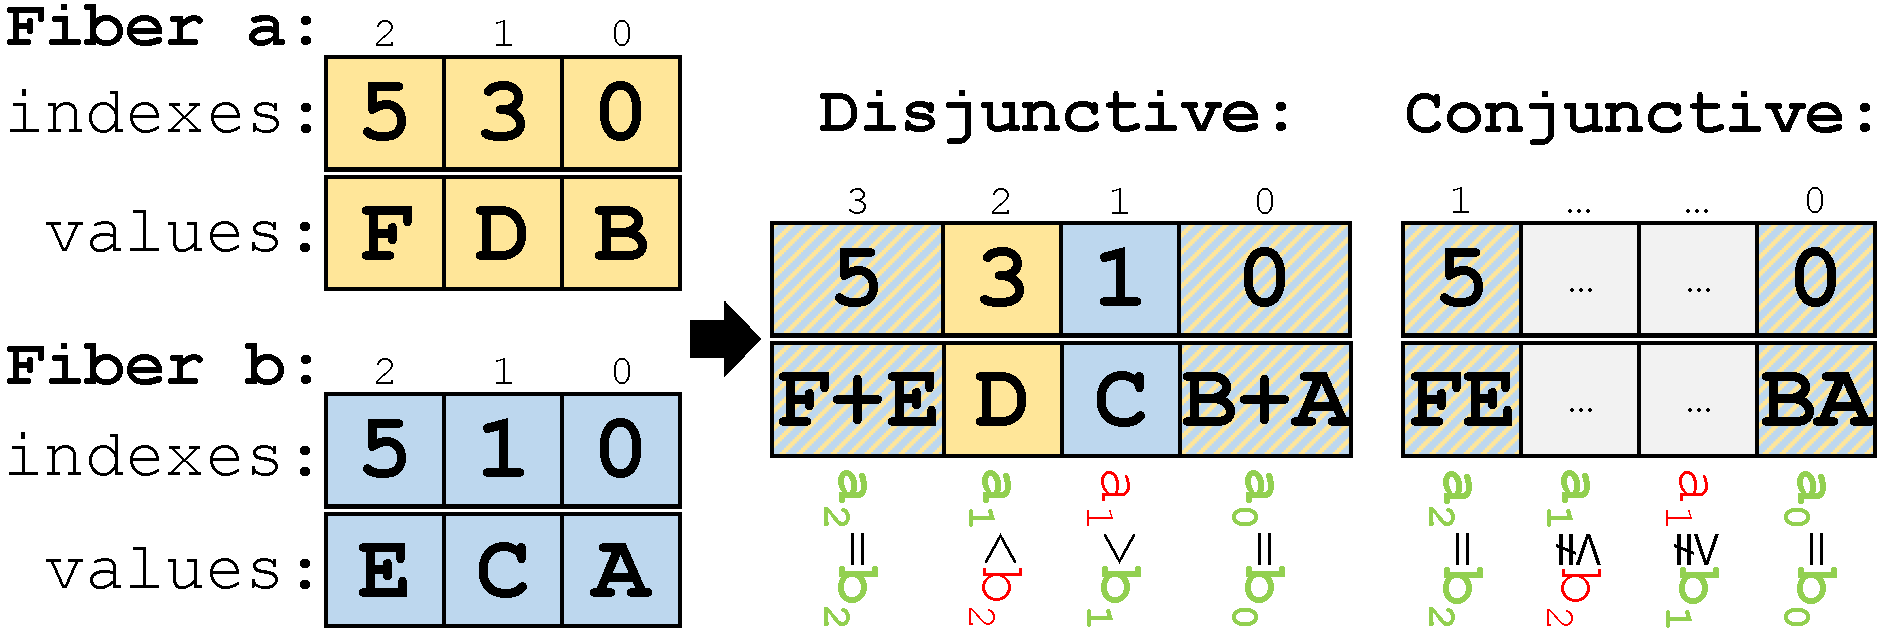
\includegraphics[width=.6\columnwidth]{img_merging_with_vals.pdf}
  \caption[Disjunctive and conjunctive merging of sparse tensors.]{Disjunctive and conjunctive merging of two tensor fibers. Disjunctive merging produces a result at a given position when at least one input fiber has a nonzero value in that position. Conjunctive merging produces a result at a given position when both fibers have a nonzero value in that position.}
  \label{fig:merging}
\end{figure}

When both tensors are sparse, fibers must be \emph{merged}. As illustrated in \Cref{fig:merging}, element-wise addition corresponds to \textit{disjunctive} merging, while element-wise multiplication corresponds to \textit{conjunctive} merging. Because $0 + x = x$, disjunctive merging co-iterates fibers and, at each step, advances the fiber with the smallest coordinate, summing values when coordinates match~\cite{hussain2022spkadd}. Conjunctive merging similarly advances fibers but outputs a value only when all fibers share the same coordinate, exploiting the fact that $0 \cdot x = 0$~\cite{hegde2019extensor}.


\begin{figure}[]
    \centering

    %-------------------- Addition --------------------%
    \begin{subfigure}[t]{0.48\linewidth}
        \centering
\begin{lstlisting}[]
CSR csr_add(const CSR& A,
    const CSR& B,
    CSR& C, // already allocated
    int m) {
  C.rowptr.resize(m + 1);
  C.rowptr[0] = 0;
  
  // For each row
  for (int i = 0; i < m; ++i) {
    int p = A.rowptr[i];
    int p_end = A.rowptr[i + 1];
    int q = B.rowptr[i];
    int q_end = B.rowptr[i + 1];

    // Until both rows have values
    while (p < p_end && q < q_end) {
      int ca = A.col[p];
      int cb = B.col[q];

      // Check column indices
      if (ca == cb) {
        // If they match, add them
        // and increment both pointers
        double v = A.val[p] + B.val[q];
        C.col.push_back(ca);
        C.val.push_back(v);
        ++p; ++q;
      } else if (ca < cb) {
        // If first is smaller
        // push it and increment
        // its pointer
        C.col.push_back(ca);
        C.val.push_back(A.val[p]);
        ++p;
      } else {
        // If first is smaller
        // push it and increment
        // its pointer
        C.col.push_back(cb);
        C.val.push_back(B.val[q]);
        ++q;
      }
    } // end co-iteration

    // Consume all other elements
    while (p < p_end) {
      C.col.push_back(A.col[p]);
      C.val.push_back(A.val[p]);
      ++p;
    }
    while (q < q_end) {
      C.col.push_back(B.col[q]);
      C.val.push_back(B.val[q]);
      ++q;
    }

    C.rowptr[i + 1] = C.col.size();
  } // end for-each row loop
}
\end{lstlisting}
        \caption{Elementwise CSR matrix addition.}
        \label{fig:csr-addition}
    \end{subfigure}
    \hfill
    %-------------------- Multiplication --------------------%
    \begin{subfigure}[t]{0.48\linewidth}
        \centering
\begin{lstlisting}[]
CSR csr_mul(const CSR& A,
    const CSR& B,
    CSR& C, // already allocated
    int m) {
  C.rowptr.resize(m + 1);
  C.rowptr[0] = 0;

  // For each row
  for (int i = 0; i < m; ++i) {
    int p = A.rowptr[i];
    int p_end = A.rowptr[i + 1];
    int q = B.rowptr[i];
    int q_end = B.rowptr[i + 1];

    // Until both rows have values
    while (p < p_end && q < q_end) {
      int ca = A.col[p];
      int cb = B.col[q];

      // Check column indices
      if (ca == cb) {
        // If they match, multiply them
        // and increment both pointers
        double v = A.val[p] * B.val[q];
        if (v != 0.0) {
          C.col.push_back(ca);
          C.val.push_back(v);
        }
        ++p; ++q;
      } else if (ca < cb) {
        // If first is smaller,
        // increment its pointer
        ++p;
      } else {
        // If second is smaller,
        // increment its pointer
        ++q;
      }
    } // End co-iteration

    C.rowptr[i + 1] = C.col.size();
  } // End for-each row loop
}
\end{lstlisting}
        \caption{Elementwise CSR matrix multiplication.}
        \label{fig:csr-multiplication}
    \end{subfigure}

    \caption[Code for elementwise addition and multiplication of two sparse matrices.]{Code for elementwise addition and multiplication of two CSR matrices.}
    \label{fig:csr-elementwise}
\end{figure}

These operations are typically implemented using \texttt{while} loops with \texttt{if}-\texttt{then}-\texttt{else} logic~\cite{taco2017oopsla}. \Cref{fig:csr-addition} shows CSR matrix addition, whereas \Cref{fig:csr-multiplication} shows CSR matrix multiplication.

Sparse-sparse and sparse-dense operations therefore expose different implementation patterns. Sparse-sparse operations must coordinate multiple compressed fibers and rely on merging to decide which coordinates produce output values. Sparse-dense operations, by contrast, often avoid explicit merging: the program scans the compressed sparse fiber and uses each sparse coordinate to look up the corresponding dense value. We refer to this pattern as \emph{scan-and-lookup}.

Scan-and-lookup is central to several workloads studied in this thesis. In SpMV using CSR, for example, the program scans the nonzeros of each sparse matrix row and uses the corresponding column indices to look up elements of the dense input vector (\Cref{fig:spmv-lookup} and \ref{fig:spmv-code}). The same pattern appears in machine learning embedding operations, where sparse IDs are scanned and used to fetch dense embedding vectors.

%%%%%%%%%%%%%%%%%%%%%%%%%%%%%%%%%%%%%%%%%%%%%%%%%%%%%%%%%%%%%%%%%%%%%%%%%%%%%%%%%%%%%%%%%%%%%%%%%%%%%%%%%%%%%%%%%%%%%%%%%%%%%%%%%%%
\subsection{Computation} \label{sec:tensor-computation} %%%%%%%%%%%%%%%%%%%%%%%%%%%%%%%%%%%%%%%%%%%%%%%%%%%%%%%%%%%%%%%%%%%%%%%%%%%%%%%%%%
%%%%%%%%%%%%%%%%%%%%%%%%%%%%%%%%%%%%%%%%%%%%%%%%%%%%%%%%%%%%%%%%%%%%%%%%%%%%%%%%%%%%%%%%%%%%%%%%%%%%%%%%%%%%%%%%%%%%%%%%%%%%%%%%%%%

After merging, fiber elements are computed and written back to memory. If the output is dense, results are stored directly. For compressed outputs, the algorithm typically proceeds in two phases: a \emph{symbolic} phase that computes or estimates the size of the output data structure, and a \emph{numeric} phase that performs floating-point computation and writes results~\cite{gao2023spgemm_survey}. A related fundamental operation is tensor \emph{reduction}, which accumulates multiple fibers into a single one~\cite{nagasaka2018spgemm,liu2021sparta}. Given a stream of coordinate--value pairs with possible coordinate repetitions, reduction produces a stream with unique coordinates by accumulating values of pairs sharing the same coordinate.

%%%%%%%%%%%%%%%%%%%%%%%%%%%%%%%%%%%%%%%%%%%%%%%%%%%%%%%%%%%%%%%%%%%%%%%%%%%%%%%%%%%%%%%%%%%%%%%%%%%%%%%%%%%%%%%%%%%%%%%%%%%%%%%%%%%
\section{Sparsity in Scientific Computing} \label{sec:sparsity-in-scientific-computing} %%%%%%%%%%%%%%%%%%%%%%%%%%%%%%%%%%%%%%%%%%%%%%%%%%%%%%%%%%%%%%%%%%%%%%%%%%%%%%%%%%%%%%%%%%%%%%%%%%%%%%%%%%%%%%%%%%%%%%%%%%%%%%%%%%%
%%%%%%%%%%%%%%%%%%%%%%%%%%%%%%%%%%%%%%%%%%%%%%%%%%%%%%%%%%%%%%%%%%%%%%%%%%%%%%%%%%%%%%%%%%%%%%%%%%%%%%%%%%%%%%%%%%%%%%%%%%%%%%%%%%%

Sparsity is a defining characteristic of many scientific workloads, arising naturally in the discretization of partial differential equations (PDEs) using finite difference (FD), finite volume (FV), and finite element (FE) methods. These discretizations couple each degree of freedom to only a few neighbors, producing large but highly sparse matrices and tensors. Exploiting sparsity is essential for reducing memory footprint and enabling large-scale simulations.

\begin{figure}
    \centering
    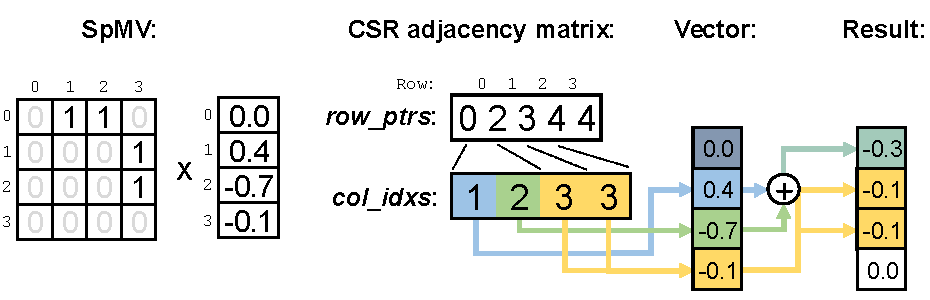
\includegraphics[width=0.8\linewidth]{img_spmv_lookup.pdf}
    \vspace{-0.5em}
    \caption[Visualization of sparse matrix-vector multiplication.]{Sparse Matrix--Vector Multiplication (SpMV), a fundamental kernel in scientific computing. The sparse adjacency matrix is stored in the Compressed Sparse Row (CSR) format~\cite{barret94csr}. Each row accumulates the vector elements referenced by its nonzero entries, which requires indirect memory accesses and results in irregular access patterns. In most cases, the fetched vector elements are also scaled by the corresponding nonzero value before being accumulated (see \Cref{fig:spmv-code}). This step is omitted here for clarity.}
    \label{fig:spmv-lookup}
\end{figure}

\begin{figure}
    \begin{lstlisting}[]
void spmv(row_ptrs: mref<? x idx>, // adj matrix CSR pointers
          col_idxs: mref<? x idx>, // adj matrix CSR indices
          nnz_vals: mref<? x f32>, // matrix nonzero values
          vec_vals: mref<? x f32>, // dense vector values
          out_vals: mref<? x f32>){ // output tensor
  // Go through all rows
  for (idx row_idx=0; row_idx<n_rows; row_idx++){
    idx ptr_beg = row_ptrs[row_idx];
    idx ptr_end = row_ptrs[row_idx+1];
    // Go through all nonzeros in a row
    for (idx ptr=ptr_beg; ptr<ptr_end; ptr++){
      f32 nnz_val = nnz_vals[ptr];
      idx col_idx = col_idxs[ptr];
      f32 vec_val = vec_vals[col_idx];
      out_vals[row_idx] += nnz_val * vec_val; }}}}
    \end{lstlisting}
    \vspace{-1em}
    \caption[Pseudocode of sparse matrix-vector multiplication.]{Pseudocode for the SpMV operation in \Cref{fig:spmv-lookup}. The outer loop iterates over CSR rows using \texttt{row\_ptrs}; the inner loop scans each row's nonzeros, loads the corresponding nonzero value and column index, and performs an indirect lookup into \texttt{vec\_vals}. The final statement accumulates the scaled dense-vector value into the output row. In the end, SpMV exposes data-dependent loop bounds and indirect load operations, which general-purpose CPUs can vectorize using gather operations.}
    \label{fig:spmv-code}
\end{figure}


Most scientific solvers revolve around sparse linear systems. Iterative methods such as Conjugate Gradient (CG), Generalized Minimal Residual (GMRES), and Bi-Conjugate Gradient Stabilized (BiCGStab) spend the majority of their time performing Sparse Matrix--Vector Multiplication (SpMV) operations, which are typically bottlenecked by irregular memory access patterns and low arithmetic intensity. Preconditioners---including algebraic multigrid (AMG) and incomplete factorizations such as incomplete LU (ILU) or incomplete Cholesky (ICC)---introduce additional sparse operations with similarly irregular behavior. \Cref{fig:spmv-lookup} presents their underlying SpMV kernel and \Cref{fig:spmv-code} its pseudocode.

Sparsity also arises in graph-based and particle-based simulations, such as molecular dynamics (MD) and network analytics, where adjacency or neighbor lists express limited physical interactions. Although sparsity reduces computational cost, it introduces irregular control flow, poor spatial locality, and load imbalance. These issues prevent modern processors---optimized for dense numerical kernels---from achieving high utilization, motivating specialized algorithms, data layouts, and hardware--software co-design efforts across scientific computing.

%%%%%%%%%%%%%%%%%%%%%%%%%%%%%%%%%%%%%%%%%%%%%%%%%%%%%%%%%%%%%%%%%%%%%%%%%%%%%%%%%%%%%%%%%%%%%%%%%%%%%%%%%%%%%%%%%%%%%%%%%%%%%%%%%%%
\section{Sparsity in Machine Learning} \label{sec:sparsity-in-machine-learning} %%%%%%%%%%%%%%%%%%%%%%%%%%%%%%%%%%%%%%%%%%%%%%%%%%%%%%%%%%%%%%%%%%%%%%%%%%%%%%%%%%%%%%%%%%%%%%%%%%%%%%%%%%%%%%%%%%%%%%%%%%%%%%%%%%%
%%%%%%%%%%%%%%%%%%%%%%%%%%%%%%%%%%%%%%%%%%%%%%%%%%%%%%%%%%%%%%%%%%%%%%%%%%%%%%%%%%%%%%%%%%%%%%%%%%%%%%%%%%%%%%%%%%%%%%%%%%%%%%%%%%%

Sparsity also plays a central role in modern machine learning models. Many models represent categorical features---such as users, products, and words---using dense embedding vectors stored in large embedding tables~\cite{glove2014emnlp}. Because the number of possible categories is extremely large, any given input activates only a small subset of entries, making interactions inherently sparse~\cite{recnmp2020isca,bigbird2024neurips,ogb2020neurips}. This section reviews the main machine learning models that leverage feature embeddings.

%%%%%%%%%%%%%%%%%%%%%%%%%%%%%%%%%%%%%%%%%%%%%%%%%%%%%%%%%%%%%%%%%%%%%%%%%%%%%%%%%%%%%%%%%%%%%%%%%%%%%%%%%%%%%%%%%%%%%%%%%%%%%%%%%%%
\subsection{Graph Machine Learning Models} \label{sec:background-graph-learning} %%%%%%%%%%%%%%%%%%%%%%%%%%%%%%%%%%%%%%%%%%%%%%%%%%%%%%%%%%%%%
%%%%%%%%%%%%%%%%%%%%%%%%%%%%%%%%%%%%%%%%%%%%%%%%%%%%%%%%%%%%%%%%%%%%%%%%%%%%%%%%%%%%%%%%%%%%%%%%%%%%%%%%%%%%%%%%%%%%%%%%%%%%%%%%%%%

A graph is formally defined as a set of nodes (vertices) and a set of edges that represent relationships between pairs of nodes. For example, in a financial network, nodes may represent economic entities such as individuals or institutions, while edges denote transactions between them. Nodes can include features such as account age, geographic region, and risk score, while edges may include features such as transaction amount, timestamp, device ID, or location.

A bank can detect fraudulent activities by analyzing the features of the nodes or edges of such a graph. Graph Neural Networks (GNNs), for instance, can infer the probability of fraud for each node by aggregating information from neighboring nodes---an operation known as \emph{graph convolution}---and processing it through neural network layers.

However, categorical features such as location or device ID cannot be directly processed by neural networks. These categories are represented as integer IDs. Since these IDs are merely indices without intrinsic numerical or relational meaning, they cannot be effectively handled using traditional machine learning techniques, which are designed for continuous numerical inputs. Graph machine learning models address this limitation by embedding structural and relational information into continuous \emph{embedding vectors}~\cite{glove2014emnlp}.

\begin{figure}
    \centering
    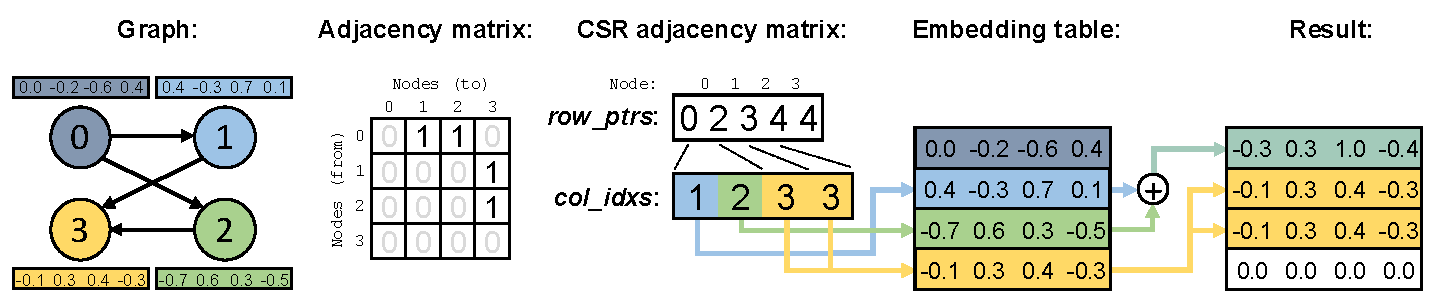
\includegraphics[width=\linewidth]{img_gnn_lookup.pdf}
    \vspace{-1em}
    \caption[Visualization of graph convolution.]{Graph convolution in GNNs implemented as a Sparse Matrix--Dense Matrix Multiplication (SpMM). The graph's sparse adjacency matrix is stored in CSR format~\cite{barret94csr}. Each node is associated with an embedding vector encoding its features. During graph convolution, each node aggregates the embedding vectors of its neighboring nodes, typically through an element-wise sum. In most cases, the fetched embedding vectors are also scaled by the corresponding nonzero value before being accumulated (see \Cref{fig:gc-code}). This step is omitted here for clarity.}
    \label{fig:gnn-lookup}
\end{figure}

\begin{figure}
    \begin{lstlisting}[]
void spmm(row_ptrs: mref<? x idx>, // adj matrix CSR pointers
          col_idxs: mref<? x idx>, // adj matrix CSR indices
          nnz_vals: mref<? x f32>, // matrix nonzero values
          emb_vals: mref<? x ? x f32>, // embedding table
          out_vals: mref<? x ? x f32>){ // output tensor
  // Go through all rows
  for (idx mtx_row_idx=0; mtx_row_idx<n_rows; mtx_row_idx++){
    idx mtx_ptr_beg = row_ptrs[mtx_row_idx];
    idx mtx_ptr_end = row_ptrs[mtx_row_idx+1];
    // Go through all nonzeros in a row
    for (idx mtx_ptr=mtx_ptr_beg; mtx_ptr<mtx_ptr_end; mtx_ptr++){
      f32 mtx_nnz_val = mtx_nnz_vals[mtx_ptr];
      idx mtx_col_idx = mtx_col_idxs[mtx_ptr];
      // Go through all elements in embedding vector
      for (idx emb_col_idx=0; emb_col_idx<emb_len; emb_col_idx++){
        f32 emb_val = emb_vals[mtx_col_idx,emb_col_idx];
        out_vals[mtx_row_idx,emb_col_idx] += mtx_nnz_val * emb_val; }}}}
    \end{lstlisting}
    \vspace{-1em}
    \caption[Pseudocode of graph convolution.]{Pseudocode for the SpMM-style graph convolution in \Cref{fig:gnn-lookup}. The outer loop iterates over graph nodes, the middle loop scans the nonzeros that identify each node's neighbors, and the inner loop traverses the embedding vector fetched for each neighbor. Compared with SpMV, the additional inner loop introduces more control-flow operations and a more regular structure that is generally leveraged for vectorization.} %This operation is similar to CSR sparse-dense matrix multiplication~\cite{aktulga2014ipdps}, although embedding vectors are not rescaled by the matrix values.}
    \label{fig:gc-code}
\end{figure}


As shown in \Cref{fig:gnn-lookup}, embedding vectors are stored in embedding tables indexed by the IDs of their corresponding vertices or edges. To perform embedding operations such as graph convolution, GNNs look up the embedding vectors of a node’s neighbors and aggregate them with, for instance, an element-wise sum. \Cref{fig:gc-code} illustrates a code example of graph convolution.

Several other graph learning models, including Message Passing (MP) models~\cite{fusedmm2021ipdps} and Knowledge Graphs (KGs)~\cite{bernerslee2001semanticweb}, leverage the same principles. MP models are a Sampled-Dense-Dense Matrix Multiplication (SDDMM) fused with an SpMM kernel~\cite{fusedmm2021ipdps}. KGs are SpMM functions that use semirings---general algebraic structures with addition and multiplication---with only one nonzero per row, requiring no segment pointers or lengths and no rescaling.

%%%%%%%%%%%%%%%%%%%%%%%%%%%%%%%%%%%%%%%%%%%%%%%%%%%%%%%%%%%%%%%%%%%%%%%%%%%%%%%%%%%%%%%%%%%%%%%%%%%%%%%%%%%%%%%%%%%%%%%%%%%%%%%%%%%
\subsection{Deep Learning Recommendation Models (DLRMs)} \label{sec:background-dlrms}  %%%%%%%%%%%%%%%%%%%%%%%%%%%%%%%%%%%%%%%%%%%%%%%%%%%%%%%%
%%%%%%%%%%%%%%%%%%%%%%%%%%%%%%%%%%%%%%%%%%%%%%%%%%%%%%%%%%%%%%%%%%%%%%%%%%%%%%%%%%%%%%%%%%%%%%%%%%%%%%%%%%%%%%%%%%%%%%%%%%%%%%%%%%%

DLRMs recommend products to users by processing a large set of categorical features under strict latency constraints~\cite{dlrm2020hpca,caches2022memsys}. They currently account for a large fraction of inference cycles in production data centers, with embedding operations consuming a significant portion of runtime~\cite{dlrm2020hpca}.

Categorical features in DLRMs are generally multi-hot, meaning they can take on multiple values (e.g., movie genres or cast). When representing these relationships as graphs, DLRMs can be viewed as a special category of graph learning models. At inference time, the embedding vectors corresponding to these values must be looked up and aggregated via operations such as an element-wise sum. High-performance implementations (1) fuse lookup and aggregation to avoid materializing intermediate results and (2) batch the categories of multiple queries to improve throughput. This operation is similar to graph convolution, although the pooling operation may differ from an element-wise sum. The \texttt{nn.EmbeddingBag} (EB) in PyTorch~\cite{pytorch2019neurips} is one such example. Unlike graph learning models, DLRMs have higher spatial locality, as discussed in \Cref{sec:characterization-and-implications}.

%%%%%%%%%%%%%%%%%%%%%%%%%%%%%%%%%%%%%%%%%%%%%%%%%%%%%%%%%%%%%%%%%%%%%%%%%%%%%%%%%%%%%%%%%%%%%%%%%%%%%%%%%%%%%%%%%%%%%%%%%%%%%%%%%%%
\subsection{Sparse Attention Mechanisms} \label{sec:background-llms} %%%%%%%%%%%%%%%%%%%%%%%%%%%%%%%%%%%%%%%%%%%%%%%%%%%%%%%%%%%%%%%%%%%%%%%%%
%%%%%%%%%%%%%%%%%%%%%%%%%%%%%%%%%%%%%%%%%%%%%%%%%%%%%%%%%%%%%%%%%%%%%%%%%%%%%%%%%%%%%%%%%%%%%%%%%%%%%%%%%%%%%%%%%%%%%%%%%%%%%%%%%%%

\begin{figure}
\centering
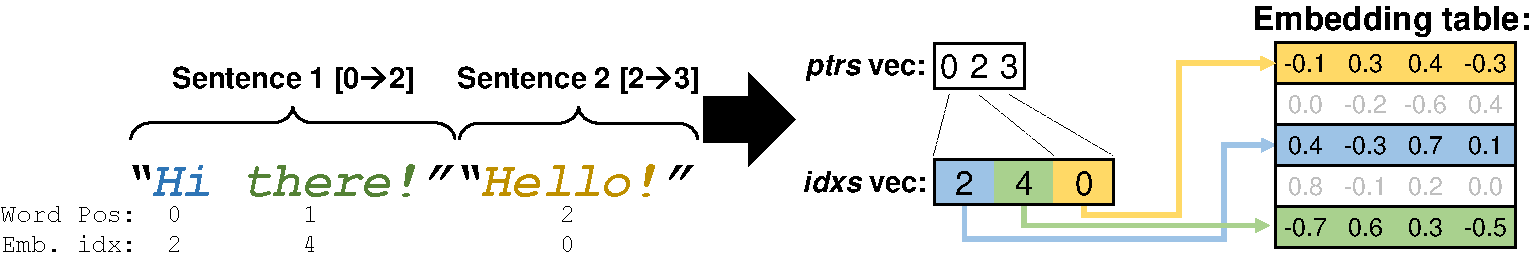
\includegraphics[width=\linewidth]{img_embedding_lookup.pdf}
\caption[Visualization of embedding lookup operations for language models.]{On the left, a batch of sentences. Each word (or subword) in a sentence is tokenized, and the tokens are compressed in a CSR-like format. These tokens are then used to look up the embedding vector from the embedding table.}
\label{fig:llm-lookup}
\end{figure}

Large Language Models (LLMs) embed text into vectors~\cite{bert2019acl}. \Cref{fig:llm-lookup} shows how categorical features are tokenized into integer IDs that index into an embedding table. Transformers such as Google's BigBird~\cite{bigbird2024neurips} sparsify the attention mechanism to compare only a selected subset of input tokens, improving memory footprint and performance on long sequences. Although this technique drastically reduces inference latency, it requires an additional step to gather embedding blocks. This gathering step is generally not fused with downstream deep neural network computation~\cite{bigbird2024neurips}, requiring only embedding lookups with no additional compute. This is similar to a \texttt{tf.gather}~\cite{tf2015whitepaper}, although it replicates blocks of embeddings from the key tensor into the query tensor.

Overall, sparse tensor workloads in both scientific computing and machine learning repeatedly exercise the same core mechanisms: compressed tensor traversal, sparse coordinate merging, and scan-and-lookup into dense operands. These mechanisms reduce storage and computation, but they also introduce irregular memory accesses, data-dependent control flow, and limited locality. The next chapter quantifies how these properties affect modern CPUs and GPUs, motivating the DAE hardware--software co-design developed in the remainder of the thesis.
